%!TEX encoding = UTF-8 Unicode
%!TEX root = ./../main.tex
%!TEX TS-program = xelatex

\chapter{Risultati sperimentali} % 5th chapter title
\label{cap:sette}
La valutazione delle \textit{performances} di un algoritmo di \ac{GI} possono essere influenzate sia positivamente che negativamente da alcuni fattori come  evidenziato in \cite{Stamina10}. Alcuni di questi fattori riguardano la complessità del \ac{DFA} target:
\begin{itemize}
\item numero di stati
\item dimensione dell'alfabeto
\item la lunghezza del più lungo dei cammini minimi dallo stato iniziale a qualunque altro stato
\item il numero di transizioni
\item il numero di transizioni totali\footnote{ (escluse quelle che vanno nello stato pozzo, altrimenti sarebbero tutte in egual numero in un \ac{DFA})}
\end{itemize}

altri il ''sample set'':
\begin{itemize}
\item Numero di campioni del \textit{training set} e del \textit{test set}
\item campioni suddetti strutturalmente completi
\end{itemize} 
Nell'effettuazione degli esperimenti è necessario tenerne conto onde evitare dei risultati pessimisticamente o ottimisticamente \textit{biased}. Per molti di questi parametri ci si è attenuti all'impostazione della competizione STAMINA \cite{Stamina10}.

\section{Dataset}
In letteratura si trovano molti algoritmi innovativi di \ac{GI} ,dei quali non si conoscono ancora le caratteristiche, che sono preventivamente testati su dei linguaggi regolari ''non banali'' ma relativamente semplici. In un secondo momento i limiti dell'algoritmo sono testati contro linguaggi più complessi che ricalcano da vicino la complessità degli automi testati nelle varie competizioni di \ac{GI} o su dataset reali. Per le finalità di questo lavoro si è scelto di perseguire questa strada.

\subsection{Tomita Dataset}
Tomita in \cite{Tomita82} definisce sette linguagi regolari, da lui usati per provare il suo algoritmo di inferenza grammaticale basato sulla tecnica di hill–climbing. Succesivamente in \cite{Dupont94}, questo insieme viene ampliato aggiungenedo altri otto linguaggi regolari. L'elenco completo dei quindici linguaggi regolari si trova in tabella \ref{tab:tom} e raggiunge un massimo di sei stati con $L_{10}$ e l'alfabeto è binario tranne in due casi, $L_{9}$ e $L_{15}$ , in cui $|\Sigma|$ = 3 . Alcuni di essi sono descritti dall’espressione regolare corrispondente. Nei casi in cui l’espressione regolare fosse troppo complicata al fine di capire immediatamente la “regolarità” del linguaggio, si è preferito fornirne una descrizione informale. Ad esempio l’espressione regolare per il linguaggio $L_6$ è $((a(ab)^{*}  (b|aa))|(b(ba)^{*} (a|bb)))^{*}$ : non è immediato riconoscere in questo caso la regolarità aritmetica posseduta dal linguaggio, costituito da tutte le stringhe in cui il numero dei caratteri $a$ differisce dal numero dei caratteri $b$ per un numero divisibile per tre.
 
\begin{table}[htp]
\centering 
\begin{tabular}{|c|M{0.75\textwidth}|} 
\hline
$L_{1}$ & $a^{*}$  \\
 \hline
 $L_{2}$ & $(ba)^{*}$  \\
 \hline
 $L_{3}$ & Ogni stringa che non contiene un numero dispari di a consecutivi dopo un numero dispari di b consecutivi  \\
 \hline   
 $L_{4}$ & Ogni stringa che non contiene la sottostringa aaa  \\
 \hline
 $L_{5}$ & Ogni stringa che contiene un numero pari di a ed un numero pari di b  \\
 \hline   
  $L_{6}$ & Ogni stringa in cui il numero di a contenute differisce dal numero di b
contenute per un numero divisibile per tre.  \\
 \hline  
 $L_{7}$ & $a^*b^*a^*b^*$  \\
 \hline
 $L_{8}$ & $a^*b$  \\
 \hline
  $L_{9}$ & $(a^*+c^*)b^*$  \\
 \hline
 $L_{10}$ & $(aa)^*(bbb)^*$  \\
 \hline
 $L_{11}$ & Ogni stringa che contiene un numero pari di a ed un numero dispari di b \\
 \hline 
 $L_{12}$ & $a(aa)^*b$ \\
 \hline     
 $L_{13}$ & Ogni stringa che contiene un numero pari di a \\
 \hline       
 $L_{14}$ & $(aa)^*ba^*$ \\
 \hline 
 $L_{15}$ & $bc^*b+ac^*a$ \\
 \hline 
\end{tabular}

 \caption[Linguaggi Tomita]{Linguaggi Tomita}
\label{tab:tom}
\end{table} 

\begin{figure}[htp]
\centering
\subfloat[$L_1$][\label{sub:tom1}]
{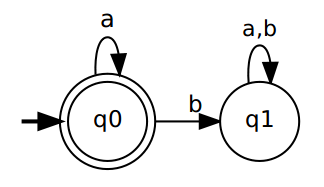
\includegraphics[width=.40\textwidth,height=4cm,keepaspectratio]{Tomita1}} \quad
\subfloat[$L_2$][\label{sub:tom2}]
{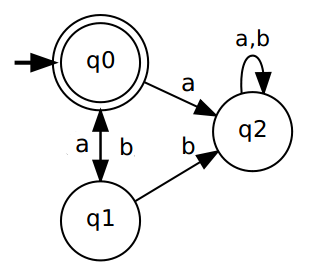
\includegraphics[width=.45\textwidth,height=4cm,keepaspectratio]{Tomita2}}\\

\subfloat[$L_3$][\label{sub:tom3}]
{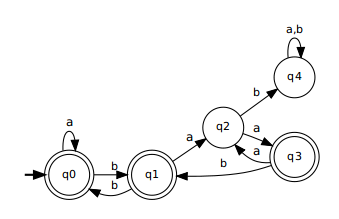
\includegraphics[width=.45\textwidth,height=4cm,keepaspectratio]{Tomita3}} \quad
\subfloat[$L_4$][\label{sub:tom4}]
{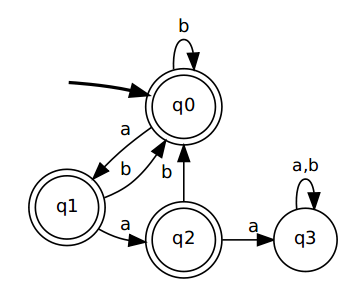
\includegraphics[width=.45\textwidth,height=4cm,keepaspectratio]{Tomita4}}\\

\subfloat[$L_5$][\label{sub:tom5}]
{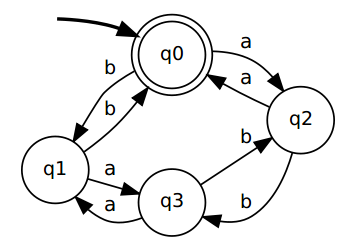
\includegraphics[width=.45\textwidth,height=4cm,keepaspectratio]{Tomita5}} \quad
\subfloat[$L_6$][\label{sub:tom6}]
{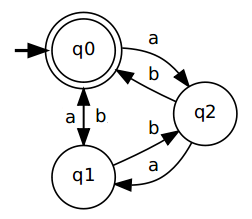
\includegraphics[width=.45\textwidth,height=4cm,keepaspectratio]{Tomita6}}\\

\subfloat[$L_7$][\label{sub:tom7}]
{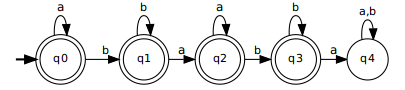
\includegraphics[width=.50\textwidth,height=4cm,keepaspectratio]{Tomita7}} \quad
\subfloat[$L_8$][\label{sub:tom8}]
{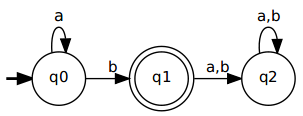
\includegraphics[width=.40\textwidth,height=4cm,keepaspectratio]{Tomita8}}\\
\caption{Linguaggi di Tomita}
\label{fig:ltom1}
\end{figure} 

\begin{figure}[htp]\ContinuedFloat
\centering
\subfloat[$L_9$][\label{sub:tom9}]
{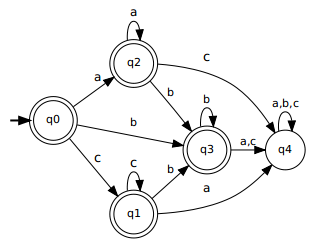
\includegraphics[width=.45\textwidth,height=4cm,keepaspectratio]{Tomita9}} \quad
\subfloat[$L_10$][\label{sub:tom10}]
{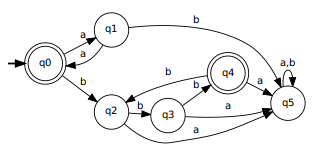
\includegraphics[width=.45\textwidth,height=4cm,keepaspectratio]{Tomita10}}\\

\subfloat[$L_11$][\label{sub:tom11}]
{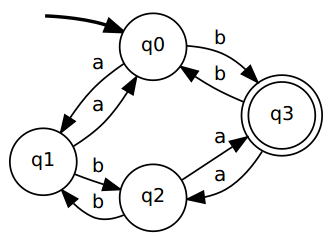
\includegraphics[width=.45\textwidth,height=4cm,keepaspectratio]{Tomita11}} \quad
\subfloat[$L_12$][\label{sub:tom12}]
{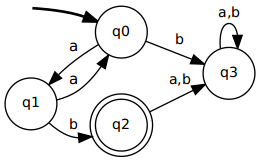
\includegraphics[width=.45\textwidth,height=4cm,keepaspectratio]{Tomita12}}\\

\subfloat[$L_13$][\label{sub:tom13}]
{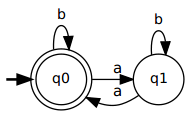
\includegraphics[width=.45\textwidth,height=4cm,keepaspectratio]{Tomita13}} \quad
\subfloat[$L_14$][\label{sub:tom14}]
{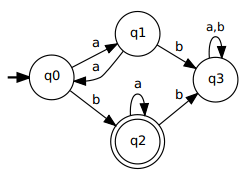
\includegraphics[width=.45\textwidth,height=4cm,keepaspectratio]{Tomita14}}\\

\subfloat[$L_15$][\label{sub:tom15}]
{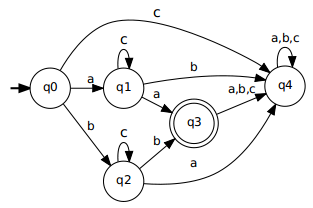
\includegraphics[width=.45\textwidth,height=4cm,keepaspectratio]{Tomita15}}

\caption{Linguaggi di Tomita}
\label{fig:ltom2}
\end{figure} 

\subsection{Dataset casuale}
Un dataset di \ac{DFA} target sicuramente più probante dalla complessità paragonabile a quella delle applicazioni reali è stato creato estraendolo in maniera casuale. La librearia GI-learning non metteva a disposizione un metodo per l'estrazione di \ac{DFA} casuali ed allo scopo si è utilizzata una libreria esterna ,la LearnLib\footnote{\href{http://www.learnlib.de/}{http://www.learnlib.de/}}. Mediante la stesura di codice ad hoc ci si è interfecciati con la LearnLib e con il metodo \textit{randomICDFA} sono stati creati i \ac{DFA} casuali, infine si è convertiti i \ac{DFA} ottenuti nel formato specifico per la lettura e il caricamento degli automi all'interno di GI-learning. 
In precedenza si è detto che le performances sugli algoritmi di  \ac{GI} sono influenzate da diversi fattori ta cui la dimensione del \ac{DFA} target e il target quindi sono parametri che vanno impostati in maniera oculata.
Sono stati creati sedici \ac{DFA} casuali con dimensione dell'alfabeto crescente che varia in $\{2,5,10,36\}$ e numeri di stati in $\{5,10,20,50\}$. Come dimensione massima dell'alfabeto si è scelto trentasei perchè corrispondente alla dimensione dell'alfabeto italiano più le dieci cifre del sistema decimale. Il limite superiore del numero di stati del \ac{DFA} target è stato fissato a cinquanta ricalcando la dimensione del \ac{DFA} target scelto   nelle varie competizioni di \ac{GI} come ABBANDINGO e STAMINA.\\
Data la complessità degli automi non è stata possibile la rappresentazione visuale come avvenuto per il dataset Tomita.


\section[Gen. campioni da DFA]{Generazione di campioni da un DFA}
\label{sec:gensam}

Se si decidesse di generare  i campioni come stringhe casuali fino a una certa lunghezza in cui ogni simbolo costituente una stringa è estratto in maniera uniforme tra tutti i simboli dell'alfabeto si  incorrerebbe nel problema che  si verrebbe ad avere un insieme non bilanciato a causa della predominanza di campioni negativi dato che tipicamente su $\Sigma^*$ sono in minoranza le stringhe accettate da un \ac{DFA}. 
Inoltre  per l'addestramento di un classificatore e anche per un algoritmo di \ac{GI} è molto importante avere un insieme caratteristico (definizione \ref{def:car}) o perlomeno un insieme di stringhe che raggiunge gran parte degli stati e delle transizioni di un \ac{DFA}.
In \cite{Stamina10} è descritto un algoritmo in grado di assicurare con altà probabilità la completezza strutturale dei campioni e di produrre campioni bilanciati. L'algoritmo effettua un \textbf{random walk} sul \ac{DFA} target e si rimanda al riferimento per i dettagli.
La proprietà dei campioni di essere strutturalmente completi(c'è solo una probabilità alta che lo siano ma non la certezza) potrebbe condurre a delle stime ottimisticamente biased dell'algoritmo \ac{ObPA} dato che in uno scenario reale invece i campioni a disposizione dell'utente sono di norma del tutto casuali (anche con random walk lo sono ma come detto in modo da esplorare tutti i percorsi del \ac{DFA})  . Nonostante ciò si è deciso  di utilizzare comunque \textit{random walk}  perchè  questa procedura è diventata uno standard de facto per generare i campioni nelle competizioni tra algoritmi riguardanti \ac{GI}.

\subsection{W-Method}
\label{sub:wme}
Per la generazione di un \textit{test set} per fare model evaluation  è improbabile che delle stringhe generate casualmente testino adeguatamente un classificatore. Quindi per la generazione del \textit{test set} dacade la valenza del discorso che campioni strutturalmente completi potrebbero condurre a sovrastimare positivamente un classificatore, assunto che rimane valido per il \textit{training set}, anzi il possedimento di questa proprietà dei dati nel \textit{test set} è ricercata per testare in maniera affidabile un classificatore che difatti approssima \ac{L}. Quindi l'utilizzo di \textit{random walk} per la generazione del \textit{test set} è assolutamente appropriato. \\   \ac{ObPA} però necessita anche del confronto dell'ipotesi intermedia \ac{H} ottenuta ad ogni \textit{round} con il \ac{DFA} target ma quest ultimo non è noto ma è approssimato da un classificatore\footnote{il classificatore approssima l'Oracolo, ma in ultima istanza ad essere approsimato è il linguaggio alias \ac{DFA} target dato che un Oracolo nel caso ideale ha il \ac{DFA} target e tramite esso risponde alle query} preliminarmente costruito tramite \ac{SVM} a partire dai campioni disponibili.   Di conseguenza l'\ac{EQ} come spiegato in [INSERIRE RIFERIMENTO SEZIONE] va implementata sottoponendo  una serie di stringhe sia al classificatore che al \ac{DFA} ipotesi \ac{H} ed è fondamentale che queste stringhe siano selezionate in maniera attenta. Estrarre le stringhe con l'algoritmo \textit{random walk} sul \ac{DFA} target in questo caso genera delle stringhe particolarmente significative ma solo per il \ac{DFA} \ac{H} ma possibilmente non rappresentative del \ac{DFA} target dato che è ignoto.\\
 E ancora sia  \textit{random smapling} che \textit{random walk} possono produrre un \textit{test set} che ha alcuni campioni in comune con il \textit{training set} con cui è stato addestrato il classificatore che approssima l'oracolo ottenendo una possibile corrispondenza mistificatoria dell' \ac{EQ}.\\
 Inoltre solo per la \textit{debug version} è possibile confrontare il \ac{DFA} finale inferito da \ac{ObPA} con il \ac{DFA} target ed anche in questo caso si ripresentano i problemi precedentemente esposti cioè eseguendo \textit{random walk} su uno dei due automi (o il target o l'ipotesi) potrebbe essere prodotto un insieme di stringhe per testare la similarità dei due linguaggi che non esplora parte dell'altro \ac{DFA} (quello su cui non si è eseguito \textit{random walk}) risultando quindi non del tutto appropriato allo scopo. Pertanto adesso è descritto l' algoritmo \textbf{W-Method} \cite{Chow78} che è esente dai problemi summenzionati.

\subsubsection{Algoritmo W-Method}

Tramite il W-Method nel contesto della \ac{GI} si realizza un' \ac{EQ} esatta impiegando solo \ac{MQ} \cite{Balanescu03}. Infatti esso crea, senza la necessità di avere il \ac{DFA} target A,  un \textit{test set}  $X$ dall'ipotesi \ac{H} in modo che se $\forall x \in X \:\:\: \lambda^{A}(x) = \lambda^{H}(x) \:\:\: \text{allora} \:\:\: A \cong \ac{H}$  (per rispondere alle \ac{MQ} lato target non è strettamente necessario avere il \ac{DFA} target ma si suppone uno scenario in cui si possa conoscere l'esito di $\lambda^{A}(x)$ senza la sua conoscenza ). Quindi il W-Method si può usare per realizzare un'\ac{EQ} in maniera esatta tramite \ac{MQ} tuttavia il numero di stringhe generate dal \textit{W-Method} può essere enorme e quindi subentrano problemi di efficienza. In questa tesi è incognito anche l'esito delle \ac{MQ} che è approssimato tramite le \ac{SVM} quindi l'\ac{EQ} realizzata tramite le stringhe prodotte dal \textit{W-Method} sarà comunque un'approsimazione. Inoltre quanto detto è vero se verificate alcune condizioni tra cui il numero esatto di stati del \ac{DFA} target   che in \ac{ObPA} non è noto nella \textit{release version} e può essere solo stimato producendo quindi un insieme di stringhe che approssimano l'equivalenza senza garantirla. Gli altri requisiti del \textit{W-Method} sono \cite{Balanescu03}:
\begin{itemize}
\item \ac{H} ed A sono deterministici
\item \ac{H} è canonico
\item Non ci sono stati irraggiungibili nè in \ac{H} nè in A
\item Si conosce $\norma{A}$
\item \ac{H} e A devono essere completamente specificati cioè da ogni stato per ogni $\Sigma$ si raggiunge uno stato che non sia lo stato pozzo(questa condizione può essere rilassata \cite{Balanescu03})
\end{itemize}
Si descrive brevemente il W-Method a grandi linee.   La ratio è che nel target potrei avere degli extra-stati che non vengono esplorati con il \textit{test set} generato con metodi classici e che potrebbero causare un comportamento indesiderato ed alterare la valutazione senza averne avvisaglie. Per questo motivo si stima in anticipo in numero di stati nel \ac{DFA} target (in modo che il test set esplori tutti gli stati del target). Per questo motivo è importante eseguire il \textit{W-Method} sul \ac{DFA} (tra ipotesi e target quando in \textit{debug version} si testa la similarità tra il target ed \ac{H}) che ha il numero minore di stati stimando gli stati dell'altro.\\
Ipotizzando in chiave espositiva che il \ac{DFA} col numero minore di stati sia \ac{H} si procede generando lo \textit{state cover} $C$ su \ac{H} cioè  $C =\{c : \forall q \in Q^{\ac{H}} \:\: \hat{\delta}^{\ac{H}}(q_\epsilon,c)=q\}$ cioè l'insieme di stringhe necessarie per raggiungere ogni stato a partire dallo stato iniziale. Due stati $q_1,q_2$ di \ac{H} sono detti \textit{W-distinguibili} se dato un insieme di stringhe $W \subseteq \Sigma^{*}  \: \:\exists x \in W : ( ( \lambda^{\ac{H}}_{q_{1}}(x) = 1 \land \lambda^{\ac{H}}_{q_{2}}(x) = 0) \lor ( \lambda^{\ac{H}}_{q_{1}}(x) = 0 \land \lambda^{\ac{H}}_{q_{2}}(x) = 1) )$ . W è detto un \textit{characterization set} se tutti gli stati distinti di \ac{H} (essendo \ac{H} minimo tutti gli stati sono distinti) presi a due a due  sono \textit{W-distinguibili}. Definito $k = \norma{A} - \norma{H}$ essere una stima (si parla di stima perchè il target A è ignoto) di quanti stati ha il target in più dell'ipotesi si ha che il \textit{test set} $Y$ è:
\begin{equation*}
Y = C(\{\epsilon\} \cup \Sigma \cup \dots \cup \Sigma^{k+1})W
\end{equation*}

Il difetto di questa tecnica è che la complessità dipende in maniera esponenziale \cite[p. 181]{Chow78} da  $\norma{A} - \norma{H}$ e quando questa differenza di stati diventa grande il metodo è ingestibile e il numero di stringhe generate dal \textit{W-Method} diventa enorme.


\subsection{Generazione dei campioni per SVM}
\label{sub:csvm}
Per effettuare l'addestramento delle \ac{SVM} è necessario creare un \textit{training set}. Anche la dimensione del \textit{training set} e del \textit{test set} è estremamente rilevante per le performances di un classificatore statistico e quindi è necessario scandagliare il comportamento dell'algoritmo al variare della dimensionalità di questi parametri. Attenendosi a quanto fatto nella competizione STAMINA \cite{Stamina10} si crea un \textit{sample set} tramite \textit{random walk}, che fornisce stringhe in maniera equamente bilanciata tra accettanti e rigettanti, sul \ac{DFA} target e da esso si estrapolano due insiemi \textbf{disgiunti}\footnote{Affinchè le performances non siano ottimisticamente biased è necessario che l'addestramento avvenga su un \textit{training set} che non ha elementi in comune con il \textit{test set}} \textit{training set} e un \textit{test set}. In STAMINA il \textit{sample set} è di dimensione 20000 e da esso si estrae un \textit{test set} di dimensione 1500 e dalle rimanenti stringhe si estrae con una procedura che non è rilevante descrivere il \textit{training set} di quattro diverse dimensioni che dipendono da un valore impostato dall'esterno ma grossolanamente si può che le quattro dimensioni del \textit{training set} sono $\{20000,10000,5000,2500\}$. Ricalcando da vicino quanto appena descritto in STAMINA si è creato con \textit{random walk} un insieme di 1500 stringhe da cui si è estratto un insieme di 1000 elementi per il \textit{test set} e 500 per il \textit{training set}. Il metodo implementato per effettuare lo \textit{splitting} è COPY\_DELETE\_SAMPLES (realizza un ''sampling without replacing'')che realizza la stratificazione (vedi Appendice \ref{sub:hol}) e funziona anche nel caso che i campioni non siano equamente bilanciati.
Rispetto a STAMINA il \textit{test set} anzichè 1500 elementi ne ha 1000 perchè è comunque un numero di campioni sufficientemente significativo e perchè per alcuni automi è risultato  complicato generare un numero elevato di campioni con \textit{random walk} come si spiegherà a breve. Per lo stesso motivo il \textit{training set} è molto ridotto rispetto a STAMINA e ciò potrebbe costituire un notevole svantaggio. Un'altra ragione per un \textit{training set} ridotto è pratico dato che SVM$^{light}$ ha dei seri problemi di convergenza quando la dimensione dell'insieme di addestramento diventa dell'ordine di 2000--3000 elementi quindi aumentarne la dimensione potrebbe rendere l'algoritmo estremamente lento. Si puntualizza che la velocità dell'algoritmo di \ac{SVM} di trovare una soluzione dipende non solo da quanti sono in numero i campioni ma anche dagli specifici dati, sia da un punto di vista di contingenza di quest ultimi che dalla difficoltà nel separarli perchè essi riflettono la complessità del linguaggio target che rappresentano cioè più il target è complesso e più è probabile che i dati siano difficili da separare con \ac{SVM}. Da un punto di vista di un'eventuale utilizzazione il limite di 500 campioni non costituisce un limite dato che i campioni in questo caso sono quelli forniti dall'utente e tipicamente non sono un numero ingente, ma ciò ha impedito di testare il comportamento di \ac{ObPA} su \textit{training set} grandi e uniformarsi a quanto fatto nelle varie competiziono di \ac{GI}.  \\ 
 Nella \textit{debug version} del codice il \textit{setting} per la generazioni dei campioni per l'addestramento è quello appena descritto; volendo simulare la  \textit{release version} senza lo sforzo di inserire dall'esterno(su file) i campioni disponibili è possibile passare  solo 500 campioni (il \textit{training set} generati sul \ac{DFA} target) senza creare il \textit{test set} nè di conseguenza dovere fare uno \textit{splitting} con stratificazione. \\
Nella \textit{release version} effettiva i campioni non vanno generati su un\ac{DFA} target perchè ignoto ma vanno inseriti dall'esterno. L'utente dovrà provvedere ad inserirli su file rispettando uno specifico formato:  
\begin{equation*}
etichetta \quad simbolo\_alfabeto \quad simbolo\_alfabeto \quad simbolo\_alfabeto \dots
\end{equation*}
Ad esempio se l'alfabeto è $\Sigma = \{0 tao 2\}$ e la stringa $tao2002tao2$ è accettante, nel file ci dovrè essere una riga siffatta:
\begin{equation*}
1 \quad tao \quad 2 \quad 0 \quad 0 \quad 2 \quad tao \quad 2
\end{equation*}
Dove il primo e unico 1 è l'etichetta per una stringa accettante, l'etichetta per una riga rigettante deve essere -1. Inoltre è necessario inserire nel file prima gli esempi positivi e poi a seguire quelli negativi. Sono ammessi duplicati perchè potrebbero essere significativi.\\

 Per alcuni linguaggi del dataset Tomita con \textit{random walk} sono stati riscontrati dei problemi nella generazione del \textit{sample set}. Si ha che \textit{random walk} nella ricerca di campioni positivi effettua un cammino probabilistico nel \ac{DFA}, che si arresta con una probabilità tale da produrre campioni che superano la profondità del \ac{DFA} (cioè di una lunghezza tale da esplorare con buona probabilità tutti gli stati del grafo); ma se il \ac{DFA} ha uno stato pozzo può accadere che molte delle stringhe casuali generate arrivino allo stato pozzo nel quale il cammino casuale termina perchè per ogni simbolo dell'alfabeto da uno stato pozzo si termina ancora in uno stato pozzo. In \ac{DFA} piccoli con pochi stati come i Tomita è altamente probabile terminare casualmente su uno stato pozzo e quindi si riescono a  generare solo pochi campioni positivi anche facendo molti tentativi ,infatti per i linguaggi incriminati che sono $L_1,L_2,L_8,L_9,L_{10},L_{12},L_{14},L_{15}$ neanche impostando una soglia altissima del numero massimo di tentativi  da fare  ci si è avvicinati ai 1500 oppure 500 campioni richiesti (la soglia è 600000 ed in alcuni casi come $L_7$ la generazione dei campioni con \textit{random walk} risulta lenta). Allora per i linguaggi suddetti malgrado quanto detto in precedenza (uniformarsi a STAMINA) si è proceduto gioco forza alla generazione casuale dei campioni. \'E importante fare notare che  i campioni positivi dei linguaggi problematici sono stati costruiti casualmente ma sfruttando sia la conoscenza della struttura dell'automa che del linguaggio evitando nella fattispecie i problemi relativi al  \textit{random sampling} per il \textit{test set} precedentemente esposti.  Ad esempio per il linguaggio $L_2$ nel caso si debbano generare $num_samples$ campioni positivi si estrae un numero casuale tra $0$ e $2*num_samples$ e il numero estratto indica quante volte consecutivamente andrà ripetuta la sottosequenza  $ba$. Considerazioni analoghe per gli altri linguaggi problematici. La generazione manuale dei campioni per i linguaggi suddetti è relativa solo ai campioni positivi, quelli negativi vengono generati ancora con \textit{random walk} (una versione modificata all'occorrenza) a partire dai campioni casuali positivi generati in precedenza\footnote{\textit{random walk} genera i campioni positivi a partire da quelli positivi effettuando un numero casuale di modifiche su di essi.}.
 
\subsection[Valutazione DFA inferito]{Comparazione di DFA target e DFA inferito da ObPA}
\label{sub:comdfa}
Nella sottosezione \ref{sub:wme} è stato detto che ,nella \textit{debug version}, quando \ac{ObPA} termina è necessario confrontare il \ac{DFA} target con il \ac{DFA} inferito dall'algoritmo \ac{ObPA}. Il \textit{test set} per effettuare il confronto va creato con il W-Method perchè rende irrilevante la presenza di eventuali campioni già usati in fase di addestramento nel \textit{test set}, genera un insieme di campioni estremamente significativo per il confronto, non necessità di un'impostazione manuale del numero di campioni nel \textit{test set} che è automaticamente tornato dal W-Method. Non sarà richiesta neanche la stima del numero di stati del \ac{DFA} target dato che quest ultimo in \textit{debug version} è noto. Nonostante i pregi evidenziati il W-Method ha originato molti problemi pratici ed è stato necessario provvedere con rimedi ad hoc. Nei seguenti casi non si usa il W-Method per la generazione dei campioni per il confronto:
\begin{enumerate}
\item \label{ite:wm1}Differenza di stati tra \ac{DFA} target e \ac{DFA} inferito maggiore di 10
\item \label{ite:wm2} \textit{Test set} creato dal W-Method troppo grande, maggior di 500000 campioni
\item \label{ite:wm3} \textit{Test set} creato dal W-Method troppo piccolo, minore di 100 campioni
\end{enumerate}
 Nel caso \ref{ite:wm1} a causa della complessità esponenziale del W-Method dipendente dalla differenza del numero di stati tra \ac{DFA} target e \ac{DFA} inferito il W-Method non termina in tempi accettabili. Nel caso \ref{ite:wm2} il W-Method termina ma ritorna un numero eccessivo di campioni che renderebbero eccessivamente lenta la fase successiva in cui si devono calcolare le statistiche sul \textit{test set} (anche se i due \ac{DFA} differiscono per pochi stati, ma hanno un numero elevato di stati il W-Method potrebbe generare un numero considerevole di stringhe. Anche per \ac{DFA} piccoli che differiscono per pochi stati ma con un grande alfabeto vengono generate tante stringhe), quindi si è fissata la soglia di 500000 campioni.  Il caso \ref{ite:wm3} deriva principalmente dalla situazione in cui il \ac{DFA} inferito da \ac{ObPA} e il \ac{DFA} target hanno lo stesso numero di stati oppure sono automi con pochi stati che differiscono per pochi stati: in tali situazioni il numero di campioni è esiguo.
 
In tutti e tre i casi si passa automaticamente  all'utilizzo di \textit{random walk} (nei casi \ref{ite:wm2} e \ref{ite:wm3} è richiesta l'esecuzione di entrambi gli algoritmi perchè per capire di essere ricaduti in uno dei casi summenzionati e passare all'esecuzione di \textit{random walk} è necessaria la preventiva esecuzione del \textit{W-Method}).  \\
Il \textit{W-Method} va sempre invocato usando come chiamante il \ac{DFA} con meno stati  (e questo può essere sia il \ac{DFA} inferito che il \ac{DFA} target).\\
La comparazione (cioè verificare la rispondenza o meno dei campioni sui due \ac{DFA}) invece avviene usando sempre il \ac{DFA} inferito come ''test'' cioè si deve testare come classifica il \ac{DFA} inferito rispetto al \ac{DFA} target ad esempio si ha un falso positivo quando il \ac{DFA} inferito classifica un campione come positivo e il \ac{DFA} target come negativo.

Quando si rientra in uno dei tre casi e si usa \textit{random walk}, siccome quest ultimo rispetto al \textit{W-Method} può essere meno attendibile, si creano 1500 campioni sia sul \ac{DFA} target che su quello inferito ; si hanno due \textit{test set}  allo scopo di non trascurare aspetti significativi dei due linguaggi.  I campioni  sono bilanciati (\textit{random walk} genera campioni bilanciati)  tuttavia quando si calcolano le statistiche sui due \textit{test set} (cioè le misure, vedi Appendice \label{sub:measure}) in entambi i casi si usa come ''test'' il \ac{DFA} inferito e ad esempio si ha un falso positivo quando il \ac{DFA} target classifica un campione come negativo e il \ac{DFA} inferito da \ac{ObPA} lo classifica come positivo. Inoltre anche se si generano 1500 stringhe bilanciate sul \ac{DFA} inferito con \textit{random walk}, esse possono risultare non bilanciate rispetto al \ac{DFA} target e questo spiega perchè nelle statistiche potrebbe comparire un numero di stringhe positive e negative differente dalla ripartizione dicotomica di 750 positive e 750 negative.\\
Una gestione particolare si è resa necessaria nel caso del Tomita dataset perchè come spiegato   nella sottosezione \ref{sub:csvm} per i linguaggi di Tomita$L_1,L_2,L_8,L_9,L_{10},L_{12},L_{14},L_{15}$  \textit{random walk} non riesce a generare i campioni e lo stesso accade in questo contesto e per essi si è dovuto generare i campioni manualmente (alla stregua di quanto fatto in fase di addestramento \ref{sub:csvm}). Inoltre per questi linguaggi di Tomita problematici si generano i 1500 campioni del \textit{test set}solo sul \ac{DFA} target, perchè il \ac{DFA} inferito da \ac{ObPA} potrebbe essere simile al target o molto diverso e quindi \textit{random walk} potrebbe ''impigliarsi'' o meno e comunque non si possono generare le stringhe accettanti manualmente perchè non si conosce il linguaggio corrispondente al \ac{DFA} inferito da \ac{ObPA}.\\

Le misure riportate in uscita (che come appena spiegato in alcuni casi sono duplici perchè relative a due \textit{test set}) sono quasi tutte descritte nell'Appendice \ref{sub:measure} e nella fattispecie sono:
\begin{itemize}
\item TP,FP,TN,TP
\item Campioni positivi e negativi (valutati sul \ac{DFA} target)
\item Accuracy
\item $Precision^{+},Recall^{+},Recall^{-}$
\item F-measure calcolata per i campioni positivi
\item Balanced Classification Rate (BCR) (misura che tiene contemporaneamente conto dei campioni positivi e negativi)
\item MCC(Mattehws correlation coeffient)
\end{itemize}        
Particolare rilevanza ai fini della valutazione come spiegato nell'Appendice \ref{sub:measure} è stata data  alla misura MCC.

Infine si puntualizza che il \textit{W-Method} pressupone due automi canonici per cui sia il \ac{DFA} inferito da \ac{ObPA} che il \ac{DFA} target vanno preventivamente minimizzati.
	  
\subsection[Gen. camp. per EQ]{Generazione dei campioni per un EQ}
\label{sub:ceq}
Per l'effettuazione di un \ac{EQ} approssimata è necessario predisporre un insieme di stringhe [INSERIRE RIFERIMENTO DOVE SI SPIEGA COME FARE UN EQ APPROSSIMATA nel capitolo 6]. L'utilizzo del \textit{W-Method} per la generazione dei campioni è una scelta naturale. In questo caso si ha un unico \ac{DFA} cioè l'ipotesi \ac{H} intermedia prodotta da \ac{ObP} e dall'altra parte si ha il classificatore inizialmente creato che approssima il \ac{DFA} target. Il \textit{W-Method} va eseguito su \ac{H} che deve essere preventivamente minimizzato dato che \ac{ObP}, come spiegato nella sottosezione \ref{sub:corret},  assicura che il \ac{DFA} finale sia minimo ma tale proprietà non è garantita per le ipotesi intermedie (a differenza dell'algoritmo $L^{*}$). \ac{ObPA} utilizza il \textit{W-Method} per generare le stringhe da \ac{H} su cui effettuare un \ac{EQ} approssimato ma nel momento in cui , per uno dei tre motivi già esposti nella sottosezione \ref{sub:comdfa}, è impossibilitato ad utilizzarlo si impiega \textit{random walk} da quel momento in poi anche per le altre eventuali ipotesi intermedie \ac{H} dato che è altamente probabile che i problemi in cui si è incorsi al passo corrente siano presenti addirittura amplificati nei successivi \textit{round} dell'algoritmo.  Essendo il numero di stati del target ignoto si utilizza un algoritmo adattivo sul numero di stati dell'ipotesi per effettuarne la previsione: basandosi sulla constatazione che al crescere del numero di stati di \ac{H} la previsione del numero di stati del target deve essere sempre più vicina a $\norma{\ac{H}}$ pena un numero di campioni esorbitante ritornato dal \textit{W-Method} si ha che 
\begin{equation*}
num\_stati\_target = floor(k * \norma{\ac{H}})
\end{equation*}
con k un valore $\in \{7,5,2.5,1.8,1.5\}$ in maniera corrispondente al superamento dei rispettivi stati di $\norma{\ac{H}} \in \{2,3,6,10,16\}$. Per meglio chiarire si ha che per esempio se $3<=\norma{\ac{H}}<6  \: \: \: k=2.5$.  Inoltre, se  $\norma{\ac{H}}>15 \: \: \: k=1.1$ 
Se le stringhe generate col W-Method sono in numero esiguo si tenta di aumentare la previsione sul numero degli stati del target e verificare se rieseguendo il \textit{W-Method} si riesce ad incrementare il numero di campioni prodotti superando la soglia minima di 100 campioni.

Nel caso si usi \textit{random walk} si cerca di generare 1500 campioni, se non ci riesce per motivi analoghi ai linguaggi Tomita si usa un \textit{test set} ridotto ma nel caso che non vengano creati neanche 100 campioni si ha il lancio di un'eccezione e la terminazione di \ac{ObPA}.


Parla del fatto che la soglia per l'eq si è impostata con un'accuracy del 90$\%$ ma non va bene questa misura. Se si ha a che fare con un \ac{DFA} come Tomita2 ad esempio che genera molte più stringhe negative che positive si ha che molte delle stringhe estratte dal W-Method se non tutte sono negative e nel primo round di \ac{ObPA} l'iptesi è il DFA che rigetta tutte le stringhe l'accuracy è al 100$\%$ e nonostante un buon classificatore si ottiene un risultato errato. Allora si è usato Matthews come misura che tenendo conto di entrambe le classi evita questo problema.

\section{ALtro}
Inserire il discorso che in debug version alla fine è comunque necessario confrontare l'ipotesi finale col target per rendersi conto del dfa inferito quanto è buono. Infatti che l'ipotesi sia verificato tramite un'equivalence query essere simile al classificatore non è sufficiente in quanto il classificatore è già di per sè un'approssimazione del target e quindi un'ipotesi che approssima bene il classificatore potrebbe non approssimare bene il target e quindi un confronto finale tra target e ipotesi è necessario. 

Inserire il discorso dell'esplosione del DFA. E che questo è dovuto anche al fatto che quando viene tornato un controesempio che non è un controesempio si fanno degli split errati. Siccome la versione implementata in librearia è ONEGlobally questa può generare più di uno split alla volta a differenza di ONELocally. Inoltre il controesempio viene sfruttato più di una volta, quindi anche un solo errore può condurre nel controesempio può condurre ad un DFA ipotesi completamente divergente dal target. Quindi potrebb essere meglio usare ONELocally che però è stato implementato ma non funzionava bene al 100 per 100.

Fai vedere le difficoltà anche nell'approssimare con OneGlobally OBP il linguaggio che il classificatore rappresenta, e non solo difficoltà nell'approssimare il linguaggio target col classificatore in addestramento.

Parla del fatto che è pssibile provare ad implementare SVM PERFCT per velocizzare il codice e provare così ad usare un training set di dimensioni maggiori e si spera migliori risultati.

Parla del caso di campioni non bilanciati che lo splitting permette di gestire campioni non bilanciati e che c'è un parametro per gestire i campioni non bilanciati. Nessun esperimento fatto su di essi.

Giustifica risultati anche perchè si approssimano anche le MQ.
Fai vedere che comunque esistono dei modelli complessi con cui si hanno buoni risultati (anche se la complessità è tutta da vedeere e non è decisa solo dagli stati dall'alfabeto e dalla profondità, ma dipende anche da quanto sono buoni i campioni estratti col random walk).
Illustra i set di esperimenti e i risultati.

Scrivi che non c'è un feedback per la bontà del classificatore come spiegato nel Capitolo 4 ma comunque si ha l'accuracy in ObPA1 e ObPA2 e il margine in ObPA3 (vedi se hai anche altro in obpa 3). E un metodo alla femminina per capire se il classificatore è buono è vedere se il classificatore viene costruito velocemente oppure SVM perde tempo. 